
Dynamic analysis tools are widely used to find bugs in
applications. They are popular among programmers because of their
precision---for many analyses, they report no false positives---and
can pinpoint the exact location of errors, down to the individual line
of code.

Perhaps the most prominent and widely used dynamic analysis tool for
C/C++ binaries is Valgrind~\cite{}. Valgrind's most popular use case
is to check memory errors, including buffer overflows, dangling
pointer errors, and memory leaks.


Buffer overflows are still one of dominant errors 
even after decades of research in this field~\cite{}: 
Four types of the CWE/SANS "Top 25 Most Dangerous Software Errors" 
~\cite{overflows1} and 
over one-third valnuerabilites of 1818 high serverity problems
reported from NIST~\cite{overflows2} are related to buffer overflows.

Since it is impossible to for programmers to write error-free programs, 
existing these problems are mainly caused by imperfection
of detection tools, which preventing the usage of them: 
either existing tools are not easy-to-use or they can not provide precise information 
or their performance
overhead are too high to be used.
A lot of tools needs programs to be annotated~\cite{} or to be recompiled~\cite{}, 
which is inconvenient for legacy software or software using third-party libraries.
Besides that, they can not provide enough information to fix problems: they can
at best point out those statements with buffer overflow problems, but without the context
why those statements are executed~\cite{}. 
Also, the performance overhead of existing tools are still too high to be
used in the production environment: two state-of-the-art tools~\cite{} are imposing over 25\%
performance overhead. 

\subsection{Contribution}
\doubletake{} is designed to tackle all these problems simultaneously for \textbf{single-threaded}
programs and it has the following contributions:

\begin{itemize}
\item \textbf{Easy-to-use}:
\doubletake{} is a drop-in library: there is no need to change the
existing operating system, to change the source code or to recompile a program,
we can simply link a program to \doubletake{} library directly or 
use the LD\_PRELOAD mechanism to link \doubletake{} beforehand.

\item \textbf{Efficiency}:
\doubletake{} designes to reduce the performance overhead for 
programs with no buffer overflows (the common case). For those programs with buffer overflows, 
\doubletake{} rollbacks and re-execute a program to locate the problems. 
With averagely 8\% performance overhead, the performance of \doubletake{} is much better than 
that of state-of-the-art tools, where imposing at least 25\% performance overhead.

Existing tools normally stop the program when an overflow is detected so that they can report 
where a problem occurs. But to detect a overflow immediately,
they instrument every memory access and introduce significant 
performance overhead (by more than 23\%). 
Completely different with these tools, \doubletake{} designes to reduce the performance overhead for 
programs with no buffer overflows (the common case) and re-executes a program deterministically
after installing watch point for those programs with buffer overflows. 
With averagely 2\% performance overhead, the performance of \doubletake{} is even better than   
that of Cruiser~\cite{overflow:Cruiser} (5\% slowdown): Cruiser utilizes an additional CPU 
to run an overflow checking thread simulataneously but can not report the locations of problems.

\item \textbf{Precision}:
\doubletake{} can report very precise and detailed information about buffer overflow problems:  
\doubletake{} reports the context of problematic memory addresses, 
which existing tools at best point out those statements with buffer overflow problems.

\item \textbf{Reliability}:
\doubletake{} does not report any false positive: all buffer overflow problems reported 
are actual buffer overflow problems. 
Besides, \doubletake{} can still work correctly even facing with segmentation fault errors.
Most of tools if not all crash unexpectedly and silently, 
without providing any useful information in case of segmentation faults 
caused by some buffer overflow and dangling pointers.
%\doubletake{} can survive these memory errors by intercepting the segmentation fault: \doubletake{}
%can even report the reason causing the segmenation fault.
\doubletake{} can find out all possible buffer overflows at a time. 
There is no need to find buffer overflows one by one: current tools
always stopped at the first error.

\item \textbf{Completeness}:
Approaches checking every memory access (relying on compiler or binary instrumentation)
may miss some buffer overflows caused by uninstrumented libraries and system calls. 
\doubletake{} can detect all kinds of buffer overflows, including those overflows caused by
system call and libraries.
  
\end{itemize} 


In order to detect a overflow immediately and report to users where a problem occurs,
existing tools instrument every memory access and introduce significant 
performance overhead (by more than 23\%). 
Completely different with these tools, \doubletake{} designes to reduce the performance overhead for 
programs with no buffer overflows (the common case) and re-executes a program when necessary to locate 
programs. 

In the beginning, \doubletake{} snapshots the state of a program by saving program counter,
registers, stack, heap state and globals. 
When buffer overflows or other memory errors are detected, \doubletake{} rollbacks a program
to its previous state: it recovers the stack, heap and globals from the saved state,
then it sets the context to saved registers (including program counter),
 making the program to be re-executed.
In order to detect those memory accesses causing buffer overflows or other errors, 
\doubletake{} installs watch points on those problematic memory addresses. 
  
For programs with no overflows(the common case), \doubletake{} only introduces the overhead 
of snapshotting a program in the beginning and checking overflows on all heap objects 
in the end, program running in the full speed most of time,  
thus it keeps the overhead to a minimum.
By using the watchpoint mechanism, \doubletake{} can report the context of buffer overflows, by presenting the whole accesses on problematic addresses, helping the user to figure out reasons for memory errors.

\subsection{Outline}
This paper talks about those related works in next section. Section 3 discusses specific mechanisms 
used by \doubletake{}. Section 4 describes some implementation details worth noting. 
Section 5 evaluates the performance and effectiveness of \doubletake{} and Section 6
discusses some problems and extending possibilities of \doubletake{}.
Section 7 concludes this paper.

\section{Overview}
\label{sec:overview}

\begin{figure}[!t]
\begin{center}
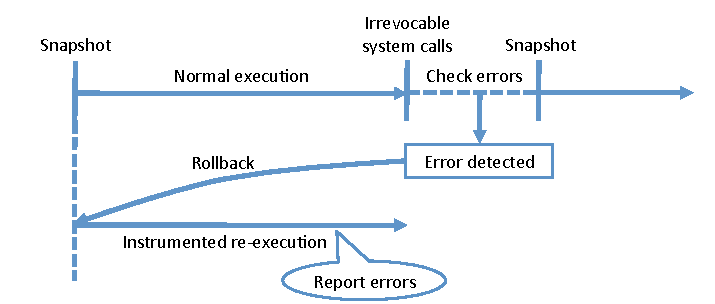
\includegraphics[width=3.3in]{doubletake/figure/overview}
\end{center}
\caption{
Overview of \doubletake{}: execution is divided into epochs at the boundary of irrevocable system calls. 
\label{fig:overview}}
\end{figure}

\doubletake{} aims to reduce the performance overhead of dynamic analyses for memory errors sharing the monotonicity: the evidence of an error is persistent and can be detected after-the-fact. As described in Figure~\ref{fig:overview}, the execution of a program is divided into epochs at irrevocable system calls, discussed in Section~\ref{sec:normal_execution}. Inside each epoch, \doubletake{} allows a program to run at full speed, with the support of checkpointing and very minimum recording overhead. \doubletake{} only checks for evidence of an error when an epoch ends. If an error is detected, \doubletake{} rolls back to the most recent checkpoint and re-execute the program to pinpoint the error.  During the re-execution phase, \doubletake{} can use higher-overhead mechanisms to pinpoint the exact cause of the error. 

Based on this framework, we have implemented three detection tools for heap buffer overflows, use-after-free errors, and memory leaks, which are described in detail in Section~\ref{sec:applications}. 

\doubletake{} employs the following core mechanisms:

\paragraph{Efficient Recording.}
At the beginning of every epoch, \doubletake{} saves a snapshot of program registers, and all writable memory. The epoch ends when the program attempts to issue an irrevocable system call, which is described in Section~\ref{} \CC{here}. \doubletake{} also records the order of thread synchronization operations to support re-execution of parallel programs. \doubletake{} records minimal system state at the beginning of each epoch (like file offsets), which allows system calls that modify this state to be undone if re-execution is required. As a result, most programs require very few epochs and program state checks. We describe the details of each application's state checks in Section~\ref{sec:applications}.

\paragraph{Precise Replay.}
During re-execution, \doubletake{} ensures that all observable system state, system call results, and memory allocations will be the same from the original run. System calls that cannot be replayed, called irrevocable system calls, must be issued at the end of an epoch after detection tools have verified that no errors have occurred. Actually, those system calls consists of the boundary of epochs, which are discussed in Section~\ref{sec:normal_execution}. In practice, most system calls can easily be replayed by handling appropriately. This ensure that most programs run very few integrity checks, and overhead remains low when errors are not detected.

\paragraph{Custom Heap Allocator.}

\doubletake{} replaces the default heap allocator with a BiBOP-style memory allocator, built on HeapLayers~\cite{heaplayers}. \DoubleTake{} pre-allocates a fixed size of memory from its underlying operating system using \texttt{mmap} system calls and satisfies memory allocations from this block by interposing all memory allocation and deallocations. Using the custom memory allocators avoids a big number of sbrk() or mmap() system calls caused by the default memory allocator. In the heap, all heap objects have the block size of {\it power of $2$}, using an object header to mark its status and size information. There is no split and merge operation on heap objects. If the size of an allocation is less than {\it power of 2}, \DoubleTake{} allocates an object with the size of next {\it power of 2}. 






\section{Applications}
\label{sec:applications}

\subsection{Shared Mechanisms}
Before the description of different applications, we listed some shared mechanisms that are used by one or multiple applications. 

\subsubsection{Canary}
\label{sec:canary}
Canary was first proposed by StackGuard~\cite{StackGuard} to find stack smashing problems by placing a canary word before the return address on stack. Those attempts to overwrite the return address should corrupt the canary word at first. Canaries are borrowed to detect buffer overflow ~\cite{overflow:purify}. They are initialized to a special value in the beginning so that modifications of those values indicates the problems. Detection tools can place canary values anywhere in heap memory. \doubletake{} introduces a bitmap to track the locations of canary values, and can check for canaries that have been overwritten. Buffer overflow detection places canary values between heap objects to detect out-of-bounds writes, and use-after-free detection fills freed objects with canaries to detect writes through dangling pointers.

\subsubsection{Watchpoints}
\label{sec:watchpoints}
Watch point mechanism relies on hardware debug registers to monitor memory accesses on specific addresses. Previous work has used this mechanism for their specific targets ~\cite{fastboundschecking, Kivati}. The main target of debug registers is to support software debuggers, e.g. gdb. A small number of watchpoints are available on modern architectures (four on x86). Each watchpoint can be configured to pause program execution when a specific byte or word of memory is accessed. \doubletake{} allows detection tools to set hardware watchpoints before re-execution. Heap Overflow detection tool can use watchpoints to find the instruction(s) responsible for overwriting a canary value.

\subsection{Applications}
\label{sec:applications}

\doubletake{} implements three important applications based on its lightweight dynamic analysis framework. Those applications are implemented in a best-effort way to show the efficiency of our framework. They are not targeted for a complete and novel solution, thus most of mechanisms are borrowed from previous work. 

\begin{figure}[!t]
\begin{center}
\includegraphics[width=3.3in]{doubletake/figure/buffer-overflow-diagram}
\end{center}
\caption{Heap organization used to provide evidence of buffer overflow errors. Object headers and unrequested space within allocated objects are filled with canaries; a corrupted canary indicates an overflow occurred.
\label{fig:buffer-overflow}}
\end{figure}

\begin{figure}[!t]
\begin{center}
\includegraphics[width=3.3in]{doubletake/figure/dangling-pointer-diagram}
\end{center}
\caption{Evidence-based detection of dangling pointer (use-after-free) errors. Freed objects are deferred in a quarantine in FIFO order and filled with canaries. A corrupted canary indicates that a write was performed after an object was freed.
\label{fig:dangling-pointer}}
\end{figure}


\subsubsection{Detection of Heap Buffer Overflows}
\label{sec:overflow}
Buffer overflows occurs when a program writes outside of the range of an allocated object. Buffer overflows can greatly affect the reliability and security of a program. 

\paragraph{Detection.}
To detect heap buffer overflows, \DoubleTake{} puts canaries before and after actual heap objects, which is described in Figure~\ref{fig:buffer-overflow}. This method is borrowed from previous work~\cite{overflow:lbc, AddressSanitizer}.
All heap objects of \doubletake{} are managed by power of two size, adding two words for canaries (16 bytes) for each heap object. For an allocation size not power of two size (a non-aligned object), \doubletake{} rounds it up to the next power of two size class, putting byte-based canaries and word-based canaries immediately after this object. This approach lets \doubletake{} catch overflows as small as one byte. 

Detection happens in the following scenario. At memory deallocation, \doubletake{} checks buffer overflows only for non-aligned objects, with size different with the power of two class. At the end of each epoch, \doubletake{} verifies integrities of all canaries by traversing the bitmap, which marks the placement of canaries and discussed in Section~\ref{sec:canaries}.  Corrupted canaries indicates heap buffer overflows. 

\paragraph{Re-execution.}
\label{sec:overflowreport}
When a program is found to have heap overflows, \doubletake{} rolls back the execution to the most recent checkpoint and re-executes this program.
To precisely identifying instructions responsible for a buffer overflow, \doubletake{} installs a watch point at the address of a corrupted canary before re-execution. When the program is re-executed, any instruction that writes to this address will trigger a debug trap (resulting in a SIGTRAP signal). \doubletake{} then reports the exact call site of trapped instructions, acquired by calling \texttt{backtrace} function. To further help programmer, \doubletake{} can also report the allocation site of an overflowed heap object. 
  
\subsubsection{Detection of Memory Leak}
\label{sec:leak}
Heap memory is leaked when it becomes inaccessible without being freed. Memory leak can greatly reduce the performance and availability of programs, which makes it one of common classes of reported bugs.

\paragraph{Detection.}
\doubletake{} detects memory leak using the same marking mechanism as conservative garbage collection ~\cite{Wilson:1992:UGC:645648.664824}. \doubletake{} marks the reachability of all heap objects: whether a heap object is reachable from the globals, the stack, and registers. Any unreachable object that has not been freed must be leaked. 

In order to compute the reachability from globals, stack, and registers, \doubletake{} starts to put all possible pointers, any eight-byte aligned value falling into the range of the heap, into a work queue. Then \doubletake{} checks all values in the queue using a breadth-first search algorithm: for each value, \doubletake{} verifies whether this value is a valid address inside a heap object; If this valid object is still non-reachable (not checked before), \doubletake{} marks it as reachable and also put all possible pointers inside this object into the work queue. After this step, this value is removed from the work queue. \doubletake{} stops when there is no value in the work queue any more. In this time, all heap objects which is reachable should have been marked. 

After the marking phase, \doubletake{} traverses the whole heap to find leaked objects, those un-reachable non-freed objects. To simplify the marking and checking phase, the status of an object, whether it is freed or reachable are marked in the object header. During this traverse, \doubletake{} recovers the status of every object to un-reachable. \doubletake{} also adds all leaked objects into a global hash table, where each leaked object also keeps information of its starting address and size. 

\paragraph{Re-execution.}
\label{sec:leakreport}
\doubletake{} uses re-execution to find allocation sites for all leaked heap objects. Re-execution proceeds as normal, with an added check in each \texttt{malloc()} function call. When a memory allocation matches the actual size and address of any leaked heap object, 
\doubletake{} reports its call stack, obtaining by using \texttt{backtrace} 
functions of \texttt{glibc} library. 

\subsubsection{Detection of Use-after-free Errors}
\label{sec:danglingpointer}
Memory use-after-free errors occur when an application continues to use a pointer after its corresponding object has been deallocated.
Writing to a freed memory can overwrite the contents of lived objects, leading to unexpected behavior.  

\paragraph{Detection.}
To detect memory use-after-free errors, 
\doubletake{} firstly delays memory re-usage of all freed objects 
by putting them into a quarantine list, same as AddressSanitizer does ~\cite{AddressSanitizer}. 
Those objects in the quarantine list are actually returned back
to the program heap when the total size of freed objects in the quarantine list are larger then a pre-defined threshold or the quarantine list is full.

In order to find evidence of memory use-after-free problems, 
\doubletake{} fills the first 128 bytes of an object, which can be adjustable, with canaries. 

Those canaries are checked before an object is returned back to the program heap or in the end of an epoch. Same as detection of buffer overflows, 
a corrupted canary indicates a use-after-free memory error and must be reported to user. 

\paragraph{Re-execution}
When a program has use-after-free memory errors, \doubletake{} re-executes this program to find out the allocation and deallocation site of corresponding objects and those instructions actually writing them.
%It is possible that multiple instructions can access an object after deallocation.  

To obtain an object's call site of allocation and deallocation, 
\doubletake{} checks starting address of each object during every memory allocation and deallocation. If an object has the same address as those use-after-free objects, its corresponding allocation/deallocation site are saved. To find out those instructions writting a freed object, 
\doubletake{} installs hardware watch points on those violating addresses, which shares the same mechanism as overflow detection.
\doubletake{} reports an use-after-free error, with its allocation site and deallocation site, in order to help programmers locate a memory use-after-free error. 

\section{Implementation} 
\label{sec:implementation}

This section describes the implementation of \doubletake{}, organized by the phases
shown in Figure~\ref{fig:phases}. 
% we should say why we have normal execution and re-execution.
Section~\ref{sec:normal_execution} firstly describes the procedure inside normal execution, which
is the common path for all programs.
Then it describes how to rollback and re-execute a program in Section~\ref{sec:re-execution}, when
there are memory errors detected.

\begin{figure*}[t] {
	\centering
	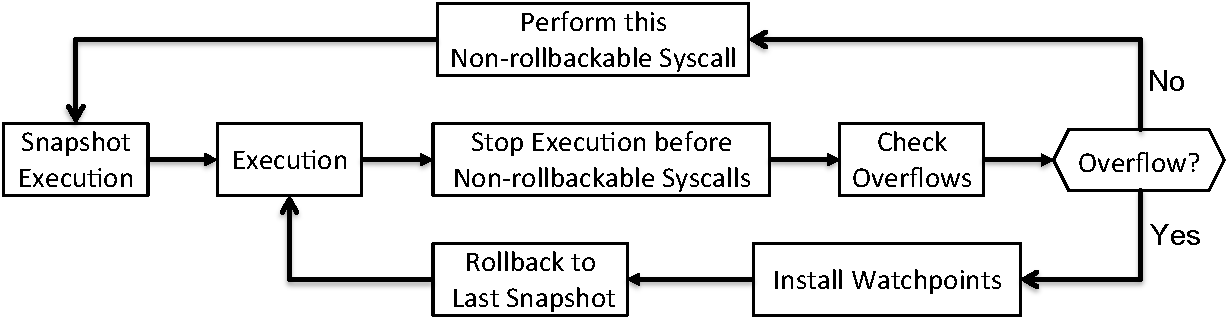
\includegraphics[width=6.5in]{figure/stopgapoverview}
	\caption{\DoubleTake{} diagram. \label{fig:phases}}
	}
\end{figure*}

\subsection{Normal Execution}
\label{sec:normal_execution}

% TODO: Fill in irrevocable system call
\doubletake{} breaks the execution of a program into multiple epochs at irrevocable system calls.
In the beginning of an epoch, \doubletake{} takes a snapshot of the program state. 
During an epoch, \doubletake{} records the program's operations to facilitate re-execution. 
An epoch ends when the program attempts to issue an irrevocable system call, such as \texttt{fork}. 
Before the system call is issued, \doubletake{} checks the program state for errors. 
When no error is detected, \doubletake{} will issue the irrevocable system call and start a new epoch.
If an error is detected, \doubletake{} switches to re-execution mode 
(described in Section~\ref{sec:re-execution}) to gather additional information about memory errors. 

\subsubsection{Starting an Epoch}
{\em Snapshot}. 
At the beginning of every epoch, \doubletake{} take a snapshot of the current program state 
so that we can rollback to this state if there are some errors detected at the end of the current epoch.
A snapshot includes the state of registers (obtained using \texttt{getcontext()}),
and all writable memory, including the globals, the stack and the program heap. 
Read-only memory, such as text segments of a program and libraries, does not need to 
be saved in the snapshot. \doubletake{} analyzes the Linux file \texttt{/proc/self/map} 
to identify the ranges of different memory mappings, including the globals and the stack.
It knows the range of the program heap because of using a customized memory allocator, which is discussed in
Section~\ref{sec:allocator}.  

To snapshot, it first saves the globals of this program and different libraries, 
and then the heap and the stack. 
In the end, it calls \texttt{getcontext} of \texttt{glibc} library to save its execution context.

{\em File Positions}. \doubletake{} records file positions of all opening files
in order to reduce the number of epochs in a program, 
which has been discussed in Section~\ref{sec:syscall}.
For a normal file, \doubletake{} calls \texttt{lseek} to acquire its file position.
For a file opened by \texttt{fopen}-like library calls,
\doubletake{} also saves its corresponding stream additionally.

\subsubsection{Executing an Epoch}
\label{sec:inepoch}
Inside an epoch, \doubletake{} intercepts those library functions involved in system calls 
and handles correspondingly according to the discussion of Section~\ref{sec:syscall}.

For checkpointable system calls, e.g., \texttt{read} and \texttt{write}, since they can 
also be called in socket communications, \doubletake{} has to check whether they 
are working on normal files. In order to speed up the checking process, \doubletake{] is using a hash map to hold file descriptors of all opening files. 
For normal files, reads and writes can be issued normally. 
For reads and writes in network communications, \doubletake{}  ends the current epochs since they are considered to be irrevocable system calls.

For recordable system calls, e.g., \texttt{gettimeofday}, \texttt{time}, and \texttt{mmap},
\doubletake{} records the results of system calls in a First-In-First-Out list, which are necessary to be replayed in re-execution phase if memory errors are detected at the end of the current epoch. 
For \texttt{open}-like library calls, \doubletake{} not only records file descriptors returned by system calls,
but also adds them to the hash map discussed above.  

For delayable system calls, e.g., \texttt{munmap} and \texttt{close}, they are added into a global 
list and are issued in the end of the current epoch after checkings of memory errors.

\subsubsection{Ending an Epoch}
At the end of each epoch, \doubletake{} checks the program state for errors. 
We have implemented error detection for heap buffer overflows (Section~\ref{sec:overflow}), 
memory leakage (Section~\ref{sec:leak}),
and memory use-after-free errors (Section~\ref{sec:danglingpointer}).

When \doubletake{} do not find any memory error, it issues all delayable system calls 
and cleans corresponding lists.
\doubletake{} also cleans recordable system calls
since there is no need to replay those system calls any more.
 
If \doubletake{} finds any memory error, it switches to the re-execution mode, discussed in Section\ref{sec:re-execution}.

\subsection{Rollback and Re-Execution}
\label{sec:re-execution}
When \doubletake{} detects an error, it uses rollback and re-execution to collect additional information to aid programmers in correcting the error. This additional information is either impossible or expensive to collect during normal execution.
In normal execution, it is impossible to know those instructions responsible for buffer overflows and 
memory usage-after-free errors if we do not check every memory access. 
Checking every memory access obviously introduces significant performance overhead, which \doubletake{} avoids. 
It is expensive to acquire call stacks for every memory allocation for detecting memory leakage, \doubletake{} leaves this operation to re-execution phase when memory leakage is detected.
By doing this, \doubletake{} enables programs to run with very low overhead until an error is detected.

\subsubsection*{Preparation}
\doubletake{} does some preparation before it rolls back and re-execute a program with memory errors. 
In order to locate instructions responsible for buffer overflows and memory usage-after-free errors,
\doubletake{} installs watch points on addresses with corrupted canaries, as described in Section~\ref{sec:applications}.
Hardware watch points are configured with debug registers, 
but these registers are only accessible to the kernel. 
Using \texttt{ptrace} function, \doubletake{} forks a child process to install watch points for current process.  

To find the allocation sites and de-allocation sites for memory usage-after-free errors and memory leakage problems, 
\doubletake{} puts all suspected heap objects into a hash map, which are checked for every memory allocation and deallocation. 

Additionally, \doubletake{} calls \texttt{lseek} to recover file positions of all opening files.

\subsubsection*{Rollback}
Regardless of the error detection being used, \doubletake{} must roll back program state 
before the epoch with errors can be re-executed. Before the program stack can be restored, \doubletake{} must switch to a temporary stack since the stack restore process may overwrite its own stack. Next, \doubletake{} restores the state of all writable memory from the epoch's snapshot. Finally, \doubletake{} restores register state with the \texttt{setcontext()} function and re-execution proceeds automatically.

\subsubsection*{Re-Execution}
The main task of re-execution is to collect additional information about different memory errors, which
have been discussed in Section~\ref{sec:applications}. 
In re-execution phase, \doubletake{} repeats the results of recordable system calls by reusing results recorded in normal execution.
For delayable system calls, \doubletake{} turns them to no-op in the re-execution phase.  


\section{Multithreading Support}
\label{sec:multithreading}

This section describes the mulithreading support of \doubletake{}.
A thread is a basic execution unit from the point of view of underlying operating system. 
The order of an execution, greatly affecting memory usage, 
is highly depending on timing, synchronization order and internal scheduling algorithm.   
Thus, it is much more difficult to achieve the target of repeatable memory 
usage for multithreading programs, which is crucial to 
precisely detect buffer overflows or other memory errors.
This section first discusses how to handle epochs in multithreading programs.
After this, it describes the design of heap allocator, suitable for repeatable memory usage.
It then discusses how to handle thread creation and exits specially. 
In the end, it describes how to guarantee deterministic synchronization in the re-execution phase,
which is also crucial for repeatable memory usage.


\subsection{Overview}
\label{sec:mtoverview}

As described in Section~\ref{sec:overview}, \doubletake{} uses irrevocable system calls as 
boundaries for epochs for multithreading programs. 
To simplify description in the following sections, a thread encountering an irrevocalbe system call is 
called as the ``Triggering-Thread''. 

When encountering an irrevocable system call, this Triggering-Thread 
has to stop all existing threads so that all other threads are in a quiecent state, which
has been described in Section~\ref{sec:stopepoch}.
Then it performs memory checkings on the heap as described in Section~\ref{sec:epochend}. 
If there is no buffer overflow, it can perform this irrevocable system call and 
start a new epoch after this system call. 
Before waking up other threads, the Triggering-Thread takes a snapshot for the shared memory at first,
including the heap and globals. 
After a thread is waken up, it only needs to take a snapshot on its own state, 
including its stack and its hardware registers. 

If there are buffer overflows, the Triggering-Thread sets up the shared memory 
for all threads at first.
It recovers the heap and globals by copying from the saved snapshot. 
Then it can wake up other threads. 
However, if the Triggering-Thread is spawed newly in current epoch, 
it has to wait for its parent to start its execution. 

\subsubsection{Epoch}
\label{sec:stopepoch}

It is the duty of a Triggering-Thread to close an epoch.
Whenever this thread meets an irrevocable system call, it has to stop other threads.
\doubletake{} utilizes the ``signal'' mechanism to stop other threads asynchronously.
It signals other threads using SIGUSR2 signal when a thread is in a safe state. 
A thread is considered to be in a unsafe state before this thread finishs a snapshot for itself,
discussed in Section~\ref{sec:threadcreation}.
After sending out all signals, this thread is waiting on a internal conditional variable.
The Triggering-Thread only starts checking buffer overflows after all threads are in quiescence.

However, this SIGUSR2 signal can also be used by user programs. 
In order to differentiate this, \doubletake{} specifically marks on 
a shared flag before signalling so that signal handler can check this in the beginning. 
If this flag is marked, this signal is issued by \doubletake{}. Otherwise, it is issued by
a user program and we can call user registered program instead. 

When other threads receive the signal from the Triggering-Thread, 
they are waiting on an internal conditional variable for instructions from the Triggering-Thread:
it can move forward to next epoch or rollback.
It is worthy noting that inside signal handler we have to utilize a different lock that has not been
used by other places. Otherwise, it is easy to cause deadlock. 

\subsubsection{Customized Heap Allocator}
\label{sec:mtheap}
In order to achive the target of repeatable memory usage, the heap allocator must be designed 
carefully. \doubletake{} first borrows a ``per-thread-heap'' idea from Hoard~\cite{Hoard}. 
\doubletake{} keeps a 1-to-1 mapping between threads and sub-heaps of customized memory allocator. 
The total number of threads and sub-heaps are pre-defined. 
A thread can only allocate memory from its own sub-heap, 
where those sub-heaps can get the memory from a pre-allocated heap 
by allocating a huge block of memory each time. 
After a sub-heap gets a block of memory, its corresponding thread always owns all objects
of this block, called as ``owner'' of this block.
This surely can cause memory blowup problem resolved by Hoard. However, it is 
not the focus of \doubletake{}.   

The ``per-thread-heap'' idea is not enough to guarantee the repeatable memory usage. 
\doubletake{} imposes several additional rules besides this.
Firstly, when \doubletake{} acquires a block of memory from the global pre-allocated heap, it must 
acquire a lock at first, which is guaranteed to be deterministic according to mechanisms 
discussed in Section~\ref{sec:sync}.
This guarantee that every new blocks of each sub-heap is repeatable for re-execution. 
Secondly, when there is a memory deallocation, this freed object can only be returned back  
to its original owner in a safe state. 
If this memory deallocation is issued by the same thread as the owner, then this freed object
can be putted into the owner's free list and be utilized immediately. 
If this memory deallocation is issued by a different thread with the owner, 
which indicates a cross-thread communication,  
then this memory
deallocation are cached into a global list, which only issued in the end of this epoch after 
all threads has been stopped. 
By doing this, we can guarantee all memory usage inside an epoch is repeatable in re-execution phase.
 
\subsection{Thread Creation and Exit}
\label{sec:threadcreation}
Tracking creations and exits of threads is very important because of the following reasons.
First, \doubletake{} has to take snapshots for different threads in the beginning. 
Second, terminination of a thread invokes \texttt{munmap} system calls directly by \pthreads{}, which
can not be intercepted.  
Third, thread creation is considered as a synchronization and has to be recorded. 
Thus, \doubletake{} intercepts \texttt{pthread\_create} calls and changes its start routine 
to a customized function. 
In this customized function, \doubletake{} can record thread creation, take a snapshot and delay thread exit to the end of current epoch. 

\subsubsection{Normal Execution}

\doubletake{} makes \texttt{pthread\_create} to call its customized function as the start routine. 
In this start routine, \doubletake{} first puts this new thread into a global map, which maintains
status of all threads. 
Then it takes a snapshot for this new thread, including stack and hardware registers. 
After this, \doubletake{} can invoke the original routine to actually perform user-defined 
thread function. 

After this user-defined thread function finishes, the control flow returns back to \doubletake{}. 
Basically, \doubletake{} should check whether this thread's parent is joining on this thread or not. 
If this thread's parent is already waiting for its termination, it simply marks the status of 
this thread to be joined and wakes up the joining thread. 
If not, this thread can wait on a thread-private conditional variables. 
\doubletake{} delays a thread exit to the end of current epoch.

\subsubsection{Re-execution}
A thread is waiting for its turn to run if a thread is created in current epoch.    

\subsection{Thread Synchronizations}

\label{sec:sync}

Different order of thread synchronizations can lead to totally different memory uage. 
In order to guarantee deterministic replay of thread synchronizations, previous work
actually forces threads to do synchronizations in a global order and
recordes both lock and unlock operations ~\cite{TERN, PRES}. 
However, forcing a global order of synchronizations can greatly 
reduce parallelism and introduce significant performance overhead.
Also, it is unnecessary to record unlock order too.

Unlike previous approaches, \doubletake{} only records local orders of synchronizations.
Synchronizations on two different synchronization variables can be performaed
in parallel. From a thread's point of view, if a program do not have a race and
all synchronizations of a thread are repeated deterministically, then
\doubletake{} can guarantee memory usage of this thread, which also guarantees to 
repeat the same buffer overflows in re-execution phase. 
If a program do have a race, forcing a global order of synchronizations in the production 
run also can not completely avoid races. This also implies that a global order 
can not always guarantee determinstic memory uage.   
\doubletake{} prefers performance for racey programs, while relying on multiple re-executions 
to repeat buffer overflows if a program does have a race problem. 

\doubletake{} records the order of \texttt{pthread\_mutex\_lock}, conditional wakenup and
different signalling functions.
Signalling functions actually calls system calls, which are handled by the procedure discussed 
in Section~\ref{sec:inepoch}.
 Conditional wakenup is actually related to \texttt{pthread\_cond\_wait},
which actually includes conditional wait and conditional wakenup phases. 
Conditional wait atomically releases mutex and waits on corresponding conditional variable, while conditional wakenup actually locks corresponding mutex before returning. 
Thus, we can turn \texttt{pthread\_cond\_wait} to two operations, \texttt{pthread\_mutex\_unlock} and
\texttt{pthread\_mutex\_lock} correspondingly. So we only record the order of conditional wakenup in
production runs. 
 
\doubletake{} also provides an option to record the order of passing a specified barrier, which it is 
not necessary to do this by default.
It is noted that \doubletake{} do not record the order of unlock operations
and conditional signal operations.
It is totally unnecessary to record unlock operations since recording the order of actual 
lock aquiring operations is enough to guarantee a deterministic replay of critical sections.  
Conditional signal and broadcast operations are skiped for the same reason. 

%why two different synchronization is not important?
How to replay this?
How to handle nested locks? 
The replaying is considerred to be two steps: we first advance thread's entry when we met a .

Maybe pseudo code for this.
 
\subsubsection{Normal Execution}
In production runs, \doubletake{} intercepts all synchronizations and 
records orders of synchronizations, such as lock, conditional waken up and signals, 
based on different synchronization variables. 
It maintains a list for each synchronization variable and records synchronization
events on its corresponding list. 
In order to quickly locate its list when a synchronization is intercepted, \doubletake{}
utilizes original synchronization variables to store addresses of list and actual synchronization
variable. 

For a synchronization event like lock, \doubletake{} records the following information:
which thread issues this synchronization event; what is the result of this synchronization.
A naive implementation is to allocate memory from internal memory allocator every time. 
However, for some applications having significant amount of synchronizations,
memory allocations to record synchronization events contributes much performance overhead. 
For example, \texttt{fluidanimate} runs several times slower because of huge amounts
of synchronizations inside. \doubletake{} uses a pre-allocated list for those recordings. 
More specifically, each thread has a pre-allocated list in the beginning of an epoch. 
When a synchronization occurs on this thread, it can get an entry from this thread and 
record a synchronization event on this entry.
Since \doubletake{} always gets an entry from current thread issuing a synchronization,
there is no need to utilize a lock, which also helps reducing overhead. 
By doing this, \doubletake{} greatly reduce performance overhead of logging synchronization
events. For example, performance overhead of \texttt{fludidanimate} are reduced to around 40\%.

 
\subsubsection{Re-execution}
As described above, for a synchronization event in a thread,
\doubletake{} allocates an entry from current thread to record this synchronization event 
and inserted it into synchronization variable's corresponding list. 
This implies that a synchronization event belongs to two lists, 
a list for all synchronizations of this synchronization variable (SyncVariableList) and 
a list for all synchronizations in a thread (ThreadSyncList). 

Reproducing synchronizations involves in manipulating these two lists using 
{\it sempaphore replay}, similar to TERN ~\cite{TERN}.
We listed the pseudocode of ``lock'' of reproduction runs in Figure~\ref{fig:lockunlock}.
\doubletake{} assigns a semaphore for each thread and controls the order 
of synchronizations based on semaphores: in lock acquisitions, 
a thread waits on its semaphore and advances ThreadSyncList after this semaphore; 
In lock releases, a thread increments the semaphore of next thread on the same 
synchronization variable.
However, \doubletake{} only records local synchronization order, instead of global order,
synchronizations replaying of \doubletake{} is much more subtle.
In order to handle those unsuccessful lock acquisitions, \doubletake{} only waits for a semaphore 
if this lock is successfully acquired in the production run. 
Also, to support nesting locks, in lock acquisitions after {\it advanceThreadSyncList()}, 
\doubletake{} signals current thread if next event of this thread is already 
in its pending list, which means that this thread should have its turn.
For lock releases, \doubletake{} adds next event of SyncVariableList to corresponding thread's 
pending list if the event is not the first event of corresponding thread instead of incrementing
its semaphore directly. 
Since performance of reproduction runs is not the main focus, only occurring for those programs 
having buffer overflows, \doubletake{} are using the same lock for all lists' manipulations to
avoid races.  




\section{Evaluation}
\label{sec:evaluation}

We evaluate \doubletake{} on a quiescent Intel Core 2 dual-processor system with 16GB of RAM running Linux 2.6.18-194.17.1.el5, and version 2.5 of \texttt{glibc}. Each processor is a 4-core 64-bit Intel Xeon, operating at 2.33GHz with a 4MB shared L2 cache a 32KB per-core L1 cache. All benchmarks are built as 64-bit executables using LLVM 3.2 with the clang front-end and \texttt{-O2} optimizations.

Our evaluation measure the runtime and memory overhead of \doubletake{}, and the effectiveness of the heap buffer overflow, memory leak, and use-after-free detectors.

\subsection{Performance Overhead}
\label{sec:perf}

\begin{figure*}[!ht]
	\begin{center}
		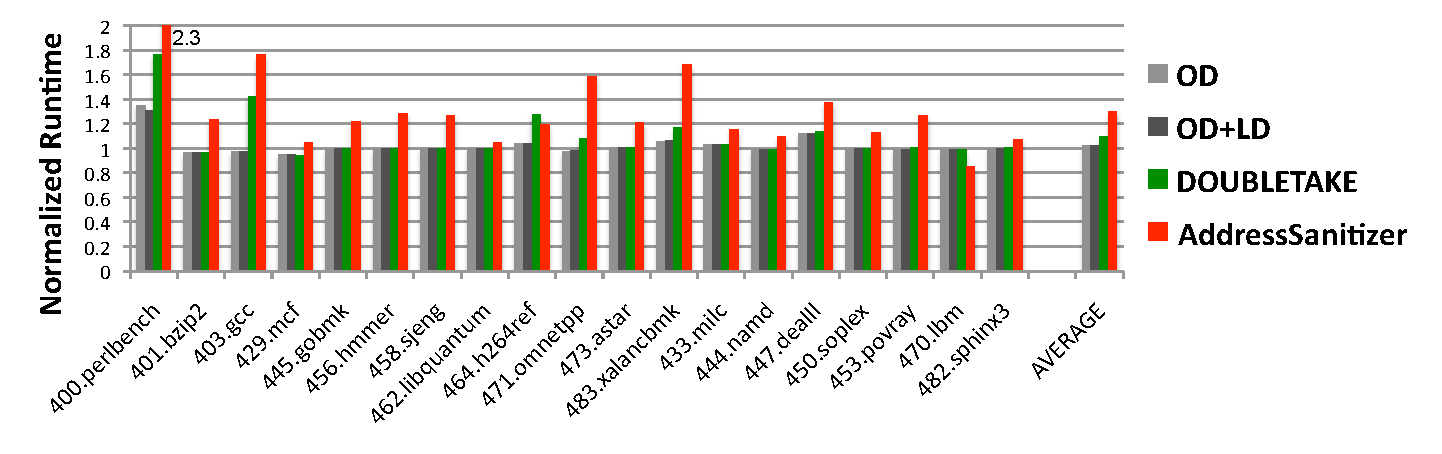
\includegraphics[width=6.5in]{doubletake/figure/perf}
	\end{center}
	\caption{This figure shows the runtime overhead of \doubletake{} (OD - Buffer Overflow Detection, LD - Leak Detection, \doubletake{} - with three detections enabled) and AddressSanitizer, normalized to each benchmark's original execution time. 
%Overhead for Valgrind is reported in Table~\ref{table:valgrind} because the results do not fit on this graph.
\label{fig:perf}}
\end{figure*}

\begin{table}[t]
	\centering
	\begin{tabular}{r|c p{0.1em} r|c}
		\textbf{Benchmark} & \textbf{Overhead} & & \textbf{Benchmark} & \textbf{Overhead} \\
		\cline{1-2} \cline{4-5}
		400.perlbench	& 20.5X	& & 458.sjeng	& 20.3X	\\
		401.bzip2		& 16.8X	& & 471.omnetpp	& 13.9X	\\
		403.gcc			& 18.7X	& & 473.astar	& 11.9X	\\
		429.mcf			& 4.5X 	& & 433.milc		& 11.0X	\\
		445.gobmk		& 28.9X	& & 444.namd		& 24.9X	\\
		456.hmmer		& 13.8X	& & 450.dealII	& 42.8X	\\
	\end{tabular}
	\caption{Valgrind's runtime overhead. \label{table:valgrind}}
\end{table}


We evaluate performance on all C and C++ SPEC CPU2006 benchmarks, 19 applications in total. We compare \doubletake{} with AddressSanitizer and Valgrind. AddressSanitizer is the previous state-of-the-art for detecting buffer overflows and use-after-free errors~\cite{AddressSanitizer}, but cannot detect memory leaks. Valgrind's Memcheck tool is widely used tool to detect buffer overflows, memory leaks, and use-after-free errors~\cite{overflow:valgrind}. 

During performance evaluation, we disable \doubletake{}'s rollback functionality to only measure the overhead of normal execution. \doubletake{} only detects memory errors of the heap, thus AddressSanitizer is run without checks on accesses to the stack and globals, and without checks on read accesses. For each benchmark, we report the average of three runs with the largest input size, except for Valgrind. We only run Valgrind once because of its slowness. 

Performance results of \doubletake{} and AddressSanitizer are shown in Figure~\ref{fig:perf}. Results for Valgrind do not fit on the graph, and are presented separately in Table~\ref{table:valgrind}. On average, \doubletake{} adds only $9\%$ overhead \emph{with all three error detectors enabled}. If \doubletake{} do not detect memory use-after-free errors, the performance overhead is under 3\% on average. AddressSanitizer slows execution by $30\%$ on average, and Valgrind has an average overhead of $19X$ on all evaluated benchmarks. Because Valgrind is running too slow, we haven't finished the evaluation on all benchmarks. Also, we kill a program if it is already running $20\times$ slower, including \texttt{400.perlbench} and \texttt{458.sjeng}. 

% difference across all different tools
For 17 out of 19 benchmarks, \doubletake{} outperforms AddressSanitizer, even with an additional memory leak detection. For 12 benchmarks, \doubletake{}'s runtime overhead is under 3\%. \doubletake{} substantially outperforms Valgrind for all benchmarks. For both \doubletake{} and AddressSanitizer,  \texttt{400.perlbench}, \texttt{403.gcc} and \texttt{447.deallIII} benchmark introduce much more performance overhead than other benchmarks. We also observe that they all introduce much more memory overhead (in terms of absolute value), according our experimental results in Table~\ref{tbl:memoryoverhead}. These significant memory overhead may reduce the ratio of cache efficiency, thus causing performance problem. 



% Difference across all different tools
From the figure, we also notice that detection of memory use-after-free adds about 6\% performance overhead averagely, although most of overhead are coming from \texttt{400.perlbench}, \texttt{403.gcc} and \texttt{464.h264ref} benchmark. As described in Section~\ref{sec:danglingpointer}, \doubletake{} has to fill every freed object up to 128 bytes with canaries and check those canaries when a freed object is released to the program heap. If an application has a big number of memory allocation and de-allocation, these operations consist of most of performance overhead. 




Table 3 shows detailed benchmark characteristics. The “Processes” column shows the number of different invocations in the input set. The number of epochs is significantly lower than the number of system calls because of \doubletake{}'s lightweight system call handling. Benchmarks with the highest overhead run a substantial number of epochs (perlbench and h264ref) and make a large number of malloc calls (gcc, omnetpp, and
xalancbmk).



\subsection{Memory Overhead}
\label{sec:memoverhead}

\begin{table}[t]
\centering
\begin{tabular}{l|c|c|c|}
\textbf{ \small Benchmark} & \textbf{\small Original} &  \textbf{\small AddressSanitizer} & \textbf{\small \doubletake{} } \\
\hline
400.perlbench & 656 &	1481 & 1977 \\
401.bzip2	& 870 &	1020 &	1003 \\
403.gcc	& 683 &	2293 &	1583 \\
429.mcf	& 1716 &	1951 &	1994 \\
445.gobmk &	28 &	137 &	58 \\
456.hmmer &	24 &	256 &	129 \\
458.sjeng & 179 & 220 &	203 \\
462.libquantum	& 66 &	144 &	131 \\
464.h264ref	& 65 &	179 &	247 \\
471.omnetpp	& 172 &	538 &	291 \\
473.astar	& 333 &	923 &	477 \\
483.xalancbmk &	428 & 1149 &	801 \\
433.milc	& 695 &	1008 &	917 \\
444.namd	& 46 &	79 &	92 \\
447.dealII	& 514 &	2496 &	1727 \\
450.soplex	& 441 &	1991 &	1654 \\
453.povray	& 3 &	133 &	50 \\
470.lbm	& 418 &	496 &	470 \\
482.sphinx3 &	45 &	181 & 98 \\
\hline
Total & 7386 & 16678 & 13906 \\
\hline
\end{tabular}
\caption{Memory Usage of \doubletake{} and AddressSanitizer(MB).\label{tbl:memoryoverhead}}
\end{table}


\begin{figure*}
\begin{center}
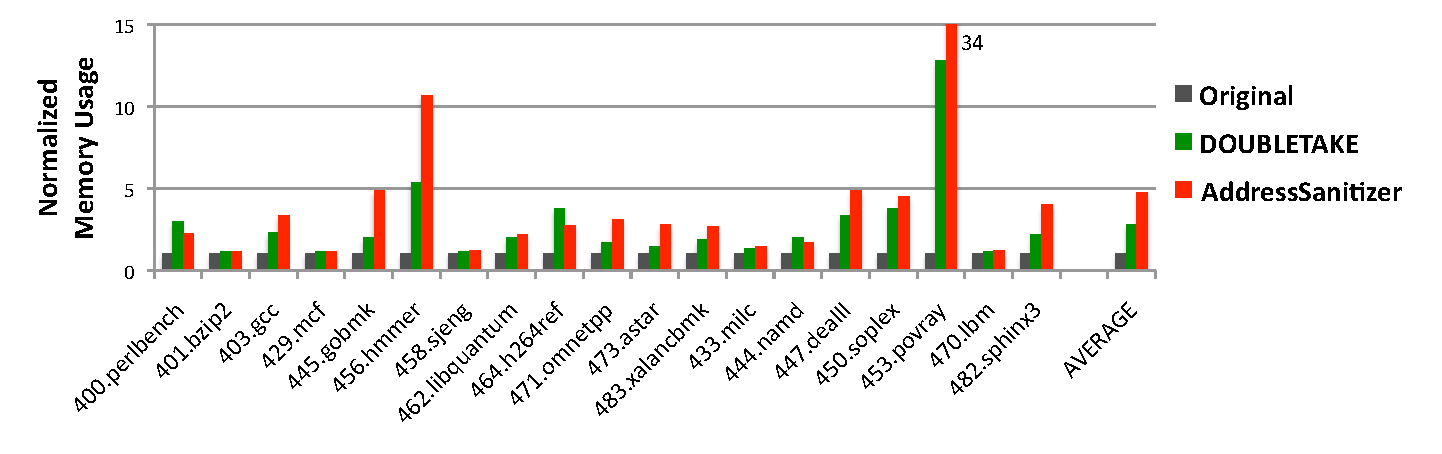
\includegraphics[width=6.5in]{doubletake/figure/memory}
\end{center}
\caption{
Memory overhead of \doubletake{} and AddressSanitizer.
\label{fig:memory}}
\end{figure*}

Memory overhead of \doubletake{} comes from the following aspects. Firstly, snapshot in the beginning of each epoch, by backing up the globals, the heap and the stack, contributes the most significant memory overhead of \doubletake{}. Snapshot can double the memory usage. However, the first snapshot happening in the beginning of a program normally doesn't take too much memory since there is no heap usage at all. Thus, this explains why \texttt{401.bzip2}, \texttt{429.mcf}, \texttt{458.sjeng},  \texttt{433.milc}, and \texttt{470.lbm} have less than $2\times$ memory overhead. Secondly, recording results of system calls introduce some memory overhead. Additionally, different applications may introduce different memory overhead. For the detection of heap buffer overflows and memory leakage, \doubletake{} adds canaries around each heap object and maintains a bit map to indicate canary locations. For the detection of memory usage-after-free errors, \doubletake{} delays memory re-usage by putting freed objects into a quarantine list, which also introduces constant additional memory overhead. 

We only evaluate the physical memory overhead here because \doubletake{} pre-allocates a huge block of heap, which is 4GB virtual memory and should not be counted as memory overhead. Also, we all only care about physical memory overhead when virtual memory overhead is practically infinite in 64bit machine. Proportional set size (PSS) in \texttt{/proc/self/smaps} reflects physical memory increase on the existing system by running an application. Thus, we periodically collect this data and use the sum of different memory mappings as total physical memory usage. We presents the normalized memory overhead of running different benchmarks in Figure~\ref{fig:memory}. We also list the actual memory usage of \doubletake{} and AddressSanitizer in Table~\ref{tbl:memoryoverhead}.

From Figure~\ref{fig:memory}, \doubletake{}'s memory overhead is 2.8$\times$, while AddressSanitizer's overhead is 4.8$\times$. For \texttt{453.povray} and \texttt{464.h264ref}, both AddressSanitizer and \doubletake{} has very high normalized memory overhead because the original memory usage of this benchmark is extremely low, only 3 and 24 megabytes. But for other benchmarks, both AddressSanitizer and \doubletake{} has memory overhead lesss than $5\times$. For all benchmarks except \texttt{400.perlbench} and \texttt{444.namd}, \doubletake{} has lower memory overhead. 
From Table~\ref{tbl:memoryoverhead}, AddressSanitizer totally spends about 20\% more memory than \doubletake{}. In total, \doubletake{} memory overhead is less than 2$\times$ of original memory usage. 

\subsection{Effectiveness}
\label{sec:effect}


We use \doubletake{} to find errors in both the SPEC CPU2006
benchmark suite and a suite of real applications.

\emph{Benchmarks.} During the evaluation of SPEC CPU2006 benchmarks, \doubletake{} detected a one-byte heap buffer overflow
 in \texttt{perlbench}, which can not be detected by AddressSanitizer. \doubletake{} also detected a big number of memory leaks in \texttt{perlbench} and \texttt{gcc}, which has been verified using Valrind.

\emph{Real Applications.} For buffer overflows, we have evaluated the effectiveness on  six real applications. \texttt{libHX} has been evaluated in previous work~\cite{overflow:Cruiser}. \texttt{bzip2}~\cite{bzip2overflow} and \texttt{vim} ~\cite{vimoverflow} are got from Red Hat Bugzilla. Other benchmarks are from bugbench~\cite{bugbench}. We especially turn global array buffer overflow in \texttt{bzip2}, \texttt{gzip}, and \texttt{polymorphy} to heap buffer overflows. \doubletake{} successfully caught all these found heap buffer overflows. The buffer overflows we observed in these applications are triggered by specific inputs, which are difficult to detect during development. \doubletake{}'s overhead is low enough to be enabled in deployment, which would make it possible to detect these bugs in the field.
\doubletake{} also detects memory leaks in \texttt{gcc-4.4.7} and \texttt{vim}.
